\chapter{Perancangan}
\label{chap:perancangan}

Bab ini menjelaskan mengenai perancangan yang disusun dari analisis yang dilakukan pada bab 3. Perancangan yang dilakukan mencakupi perancangan kelas, diagram \textit{sequence}, serta penjelasan mengenai hasil analisis yang tidak mungkin diimplementasikan dan cara lain yang dilakukan untuk mendapatkan hasil yang serupa.



\section{Perancangan Kelas}
\label{sec:perancangan_kelas}

Gambar \ref{fig:DetailedClassDiagram} menjelaskan mengenai kelas-kelas dalam perangkat lunak yang dibuat. Beberapa kelas utama yang perlu dijelaskan antara lain:

\par{\textbf{MainPage} : Kelas ini merupakan kelas yang berperan sebagai tampilan utama aplikasi. Atribut-atribut yang dimiliki oleh kelas ini adalah:
    \begin{itemize}
        \item{cpd\\Atribut untuk menyimpan \textit{instance} CaptivePortalDetector.}
        \item{timeoutTimer\\Atribut untuk menyimpan timer yang digunakan untuk menghitung \textit{connection timeout}.}
        \item{loaded\\Atribut untuk menyimpan status \textit{loading} suatu halaman.}
    \end{itemize}
    Metode-metode yang dimiliki oleh kelas ini adalah:
    \begin{itemize}
        \item{setup\\Metode ini digunakan untuk melakukan \textit{setup} awal saat aplikasi dieksekusi. Fungsinya adalah untuk menyimpan \textit{instance} CaptivePortalDetector dan memanggil metode setup() pada \textit{instance} tersebut.}
        \item{MainWebView\_LoadCompleted\\Metode ini dipanggil saat WebView selesai melakukan loading halaman. Fungsinya adalah untuk memanggil metode onLoad() pada CaptivePortalDetector.}
        \item{MainWebView\_NavigationStarting\\Metode ini dipanggil saat WebView baru akan memulai navigasi ke halaman baru. Fungsinya adalah untuk memulai \textit{timer} untuk \textit{timeout} dan memasukkan objek ScriptNotifyHandler.}
        \item{MainWebView\_NewWindowRequested\\Metode ini dipanggil saat WebView melakukan \textit{request} untuk membuka window baru. Fungsinya adalah untuk memanggil metode queueUri() pada CaptivePortalDetector.}
        \item{MainWebView\_NavigationCompleted\\Metode ini dipanggil saat WebView selesai melakukan navigasi ke halaman baru, namun belum selesai melakukan loading halaman tersebut. Fungsinya adalah untuk melakukan \textit{override} fungsi-fungsi JavaScript seperti window.open() dan open() agar bisa diakses dari JavaScript tanpa aksi langsung dari pengguna.}
    \end{itemize}
}

\begin{figure}[!htb]
    \centering
    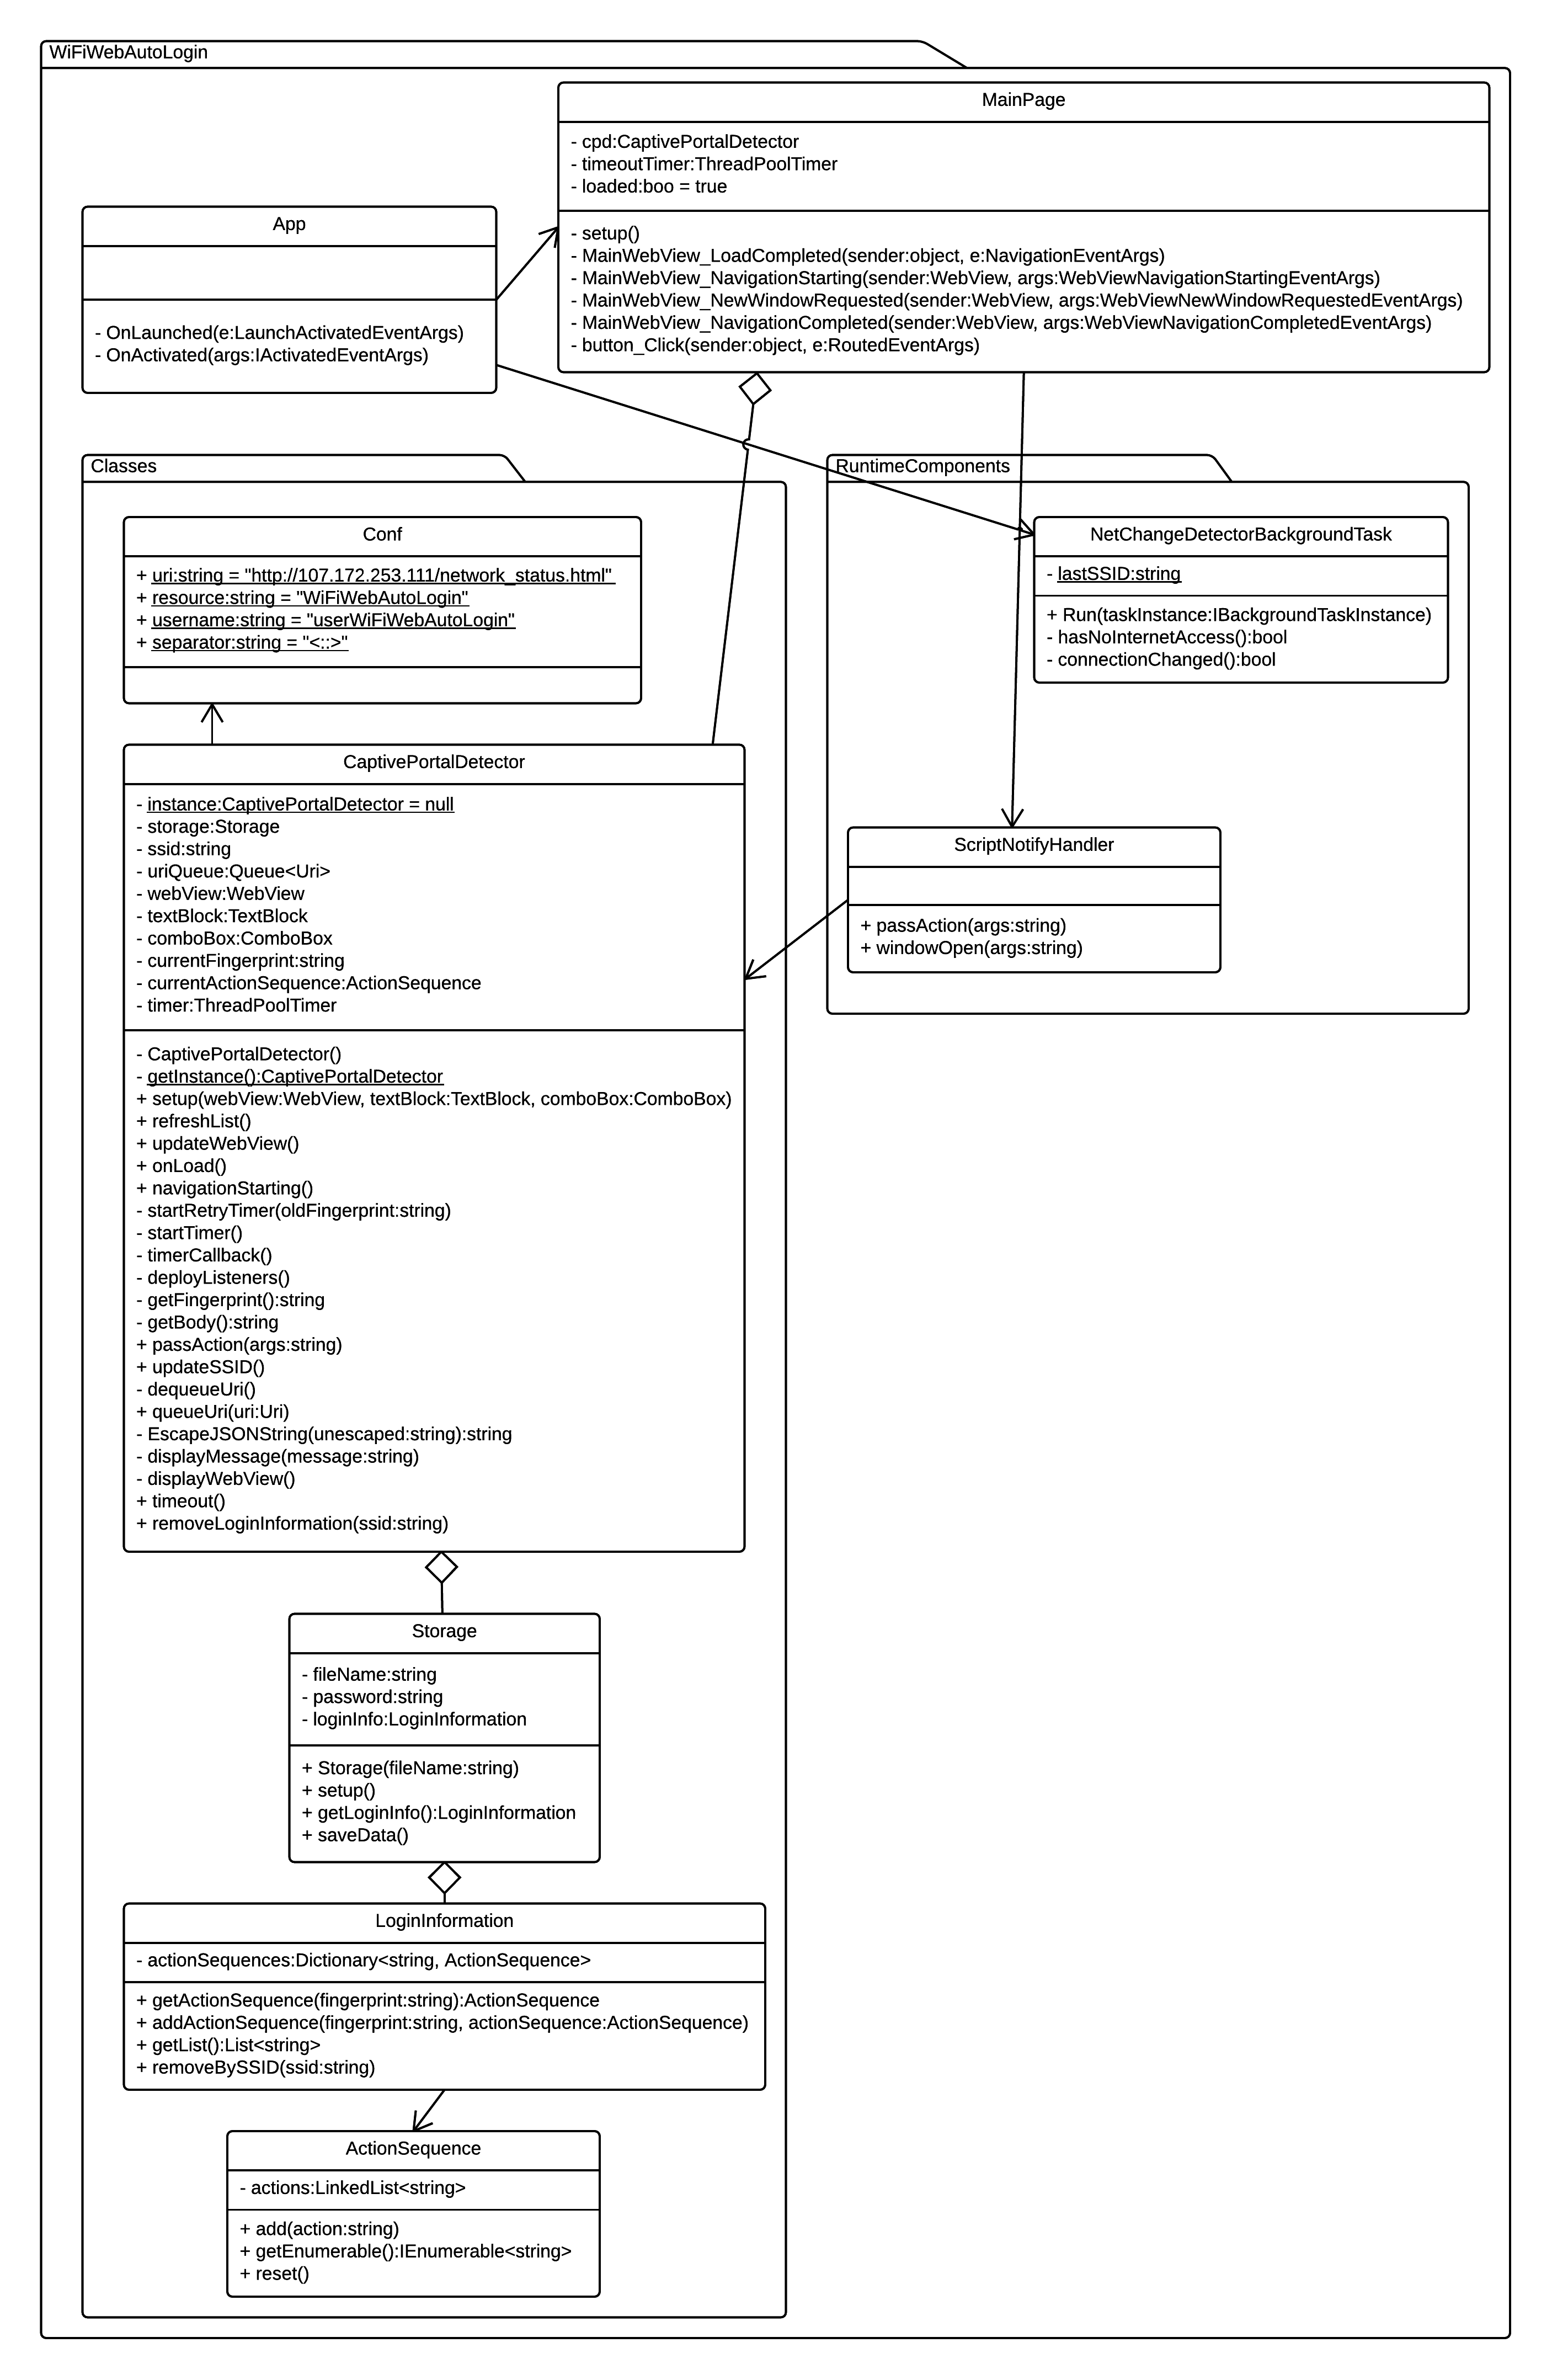
\includegraphics[scale=0.63]{Gambar/DetailedClassDiagram.png}
    \caption[Diagram Kelas Rinci.]{Diagram Kelas Rinci.} 
    \label{fig:DetailedClassDiagram}
\end{figure}

\par{\textbf{NetChangeDetectorBackgroundTask} : Kelas ini merupakan kelas yang digunakan untuk melakukan deteksi perubahan jaringan yang nantinya digunakan untuk menampilkan notifikasi apabila terdeteksi adanya jaringan yang terhubung tanpa adanya internet. Atribut yang dimiliki oleh kelas ini adalah:
    \begin{itemize}
        \item{lastSSID\\Atribut ini menyimpan SSID terakhir yang nantinya akan dibandingkan dengan SSID terbaru untuk mendeteksi adanya perubahan SSID.}
    \end{itemize}
    Metode-metode yang dimiliki oleh kelas ini adalah:
    \begin{itemize}
        \item{Run\\Metode ini dipanggil saat Windows mengalami perubahan jaringan. Fungsinya adalah untuk menampilkan notifikasi apabila kondisi \texttt{connectionChanged() \&\& lastSSID!=null \&\& hasNoInternetAccess()} terpenuhi.}
        \item{hasNoInternetAccess\\Metode ini digunakan untuk medeteksi tidak adanya akses internet menggunakan API yang diberkan oleh UWP.}
        \item{conectionChanged\\Metode ini digunakan untuk medeteksi perubahan SSID.}
    \end{itemize}
}

\par{\textbf{ScriptNotifyHandler} : Kelas ini merupakan kelas yang digunakan untuk menghubungkan sisi javascript pada WebView dengan kode C\#. Metode-metode yang dimiliki oleh kelas ini adalah:
    \begin{itemize}
        \item{passAction\\Metode ini dipanggil saat \textit{listener} yang sudah disisipkan ke dalam WebView mendeteksi \textit{action} yang dapat direkam. \textit{Action} yang direkam berupa teks yang berisi kode javascript yang dapat mereplikasi \textit{action} tersebut.}
        \item{windowOpen\\Metode ini dipanggil saat javascript pada WebView memanggil fungsi window.open atau fungsi open.}
    \end{itemize}
}

\par{\textbf{CaptivePortalDetector} : Kelas ini merupakan kelas utama yang berfungsi untuk melakukan deteksi \textit{captive portal}, menyisipkan kode \textit{listener} pada WebView, merekam \textit{action sequence} yang dilakukan oleh pengguna, dan menjalankan kembali \textit{action sequence} yang sudah tersimpan. Kelas ini menggunakan \textit{design pattern} singleton agar kelas-kelas lainnya bisa mengakses \textit{instance} yang sama pada setiap \textit{session}. Atribut yang dimiliki oleh kelas ini adalah:
    \begin{itemize}
        \item{instance\\Atribut ini menyimpan \textit{instance} CaptivePortalDetector.}
        \item{storage\\Atribut ini menyimpan objek Storage yang digunakan untuk menyimpan dan mengakses informasi login.}
        \item{ssid\\Atribut ini menyimpan SSID saat ini.}
        \item{uriQueue\\Atribut ini menyimpan queue Uri yang perlu diakses.}
        \item{webView\\Atribut ini menyimpan WebView yang digunakan untuk melakukan deteksi \textit{captive portal}.}
        \item{textBlock\\Atribut ini menyimpan TextBlock yang digunakan untuk menampilkan pesan kepada pengguna.}
        \item{comboBox\\Atribut ini menyimpan ComboBox yang digunakan untuk menampilkan daftar SSID yang sudah tersimpan kepada pengguna.}
        \item{currentFingerprint\\Atribut ini menyimpan fingerprint saat ini.}
        \item{currentActionSequence\\Atribut ini menyimpan ActionSequence yang terkait dengan fingerprint saat ini.}
        \item{timer\\Atribut ini menyimpan timer yang digunakan untuk mengatur waktu akses Uri dalam uriQueue.}
    \end{itemize}
    Metode-metode yang dimiliki oleh kelas ini adalah:
    \begin{itemize}
        \item{getInstance\\Metode ini digunakan untuk mendapatkan \textit{instance} dari CaptivePortalDetector.}
        \item{setup\\Metode ini digunakan untuk melakukan \textit{setup} awal yang menyimpan WebView, TextBlock, dan ComboBox ke dalam \textit{instance} CaptivePortalDetector.}
        \item{refreshList\\Metode ini digunakan untuk melakukan \textit{refresh} tampilan ComboBox.}
        \item{updateWebView\\Metode ini digunakan untuk menentukan melakukan deteksi \textit{captive portal} jika terhubung dengan koneksi WiFi, atau menampilkan pesan kepada pengguna juka tidak terhubung dengan koneksi WiFi.}
        \item{onLoad\\Metode ini dipanggil saat WebView sudah selesai melakukan \textit{loading} halaman. Fungsinya adalah untuk melakukan deployListener(), menjalankan aksi-aksi yang sudah terekam pada informasi login, dan mendeteksi sudah atau belum terjadinya koneksi dengan internet.}
        \item{navigationStarting\\Metode ini dipanggil saat WebView mulai melakukan navigasi ke halaman baru. Fungsinya adalah untuk membatalkan timer untuk membuka halaman-halaman popup dari halaman sebelumnya.}
        \item{passAction\\Metode ini digunakan untuk menyimpan \textit{action} yang dikirimkan oleh ScriptNotifyHandler ke dalam currentActionSequence.}
        \item{updateSSID\\Metode ini digunakan untuk mendapatkan SSID terbaru.}
        \item{queueUri\\Metode ini digunakan untuk memasukkan Uri baru ke dalam uriQueue.}
        \item{timeout\\Metode ini digunakan untuk menyatakan bahwa terjadi \textit{connection timeout}.}
        \item{removeLoginInformation\\Metode ini digunakan untuk menghapus seluruh informasi login yang terkait dengan SSID tertentu.}
    \end{itemize}
}

\par{\textbf{Storage} : Kelas ini digunakan untuk menyimpan informasi login dan password yang digunakan untuk melakukan enkripsi. Atribut yang dimiliki oleh kelas ini adalah:
    \begin{itemize}
        \item{fileName\\Atribut ini menyimpan nama file yang digunakan untuk menyimpan informasi login yang terenkripsi.}
        \item{password\\Atribut ini menyimpan password yang digunakan untuk melakukan enkripsi.}
        \item{loginInfo\\Atribut ini menyimpan objek LoginInformation yang digunakan untuk menyimpan seluruh informasi login.}
    \end{itemize}
    Metode-metode yang dimiliki oleh kelas ini adalah:
    \begin{itemize}
        \item{setup\\Metode ini digunakan untuk melakukan \textit{setup} awal seperti membuka file dan melakukan dekripsi.}
        \item{getLoginInfo\\Metode ini digunakan untuk mendapatkan objek LoginInformation.}
        \item{saveData\\Metode ini digunakan untuk menyimpan data yang ada pada objek LoginInformation ke dalam file dan melakukan enkripsi pada file tersebut.}
    \end{itemize}
}

\par{\textbf{LoginInformation} : Kelas ini digunakan untuk merepresentasikan informasi login. Atribut yang dimiliki oleh kelas ini adalah:
    \begin{itemize}
        \item{actionSequences\\Atribut ini merupakan pasangan \textit{key-value} antara suatu fingerprint dengan ActionSequence.}
    \end{itemize}
    Metode-metode yang dimiliki oleh kelas ini adalah:
    \begin{itemize}
        \item{getActionSequence\\Metode ini digunakan untuk mendapatkan ActionSequence berdasarkan fingerprint tertentu.}
        \item{addActionSequence\\Metode ini digunakan untuk menambahkan ActionSequence untuk fingerprint tertentu.}
        \item{removeBySSID\\Metode ini digunakan untuk menghapus ActionSequence milik fingerprint tertentu.}
        \item{getList\\Metode ini digunakan untuk mendapatkan daftar SSID yang sudah direkam.}
    \end{itemize}
}

\par{\textbf{ActionSequence} : Kelas ini digunakan untuk merepresentasikan urutan \textit{action}. Atribut yang dimiliki oleh kelas ini adalah:
    \begin{itemize}
        \item{actions\\Atribut ini merupakan daftar \textit{action} yang berupa kode javascript.}
    \end{itemize}
    Metode-metode yang dimiliki oleh kelas ini adalah:
    \begin{itemize}
        \item{add\\Metode ini digunakan untuk menambahkan \textit{action} ke dalam daftar ini.}
        \item{getEnumerable\\Metode ini digunakan untuk mendapatkan enumerable dari daftar \textit{actions}, sehingga mempermudah eksekusi \textit{actions}.}
        \item{reset\\Metode ini digunakan untuk menghapus seluruh \textit{action} yang ada pada daftar ini.}
    \end{itemize}
}



\section{Perancangan Algoritma dan Struktur Data}
\label{sec:perancangan_algoritma_dan_struktur_data}

Sub-bab ini menjelaskan mengenai perancangan algoritma untuk melakukan deteksi \textit{captive portal}, struktur data dan format \textit{fingerprint}, serta struktur data untuk menyimpan informasi login.

\subsection{Algoritma Deteksi \textit{Captive Portal}}
\label{subsec:algoritma_deteksi_captive_portal}

Algoritma yang digunakan untuk melakukan deteksi \textit{captive portal} adalah sebagai berikut:

\hfill

\begin{algorithm}[H]
    \If{Network Detected and No Internet Connection}{
        Ask user to run application via notification\;
        \If{"Yes" button clicked}{
            Access a web page which can only be opened if there is an internet connection\;
            \If{Redirected}{
                Captive portal detected\;
            }
        }
    }
\end{algorithm}

\hfill

Algoritma di atas menjelaskan deteksi \textit{captive portal} dilakukan dengan melakukan deteksi jaringan yang tidak terhubung dengan internet. Jika ditemukan jaringan yang tidak terhubung dengan internet, maka akan muncul notifikasi yang memungkinkan pengguna untuk menjalankan perangkat lunak. Saat perangkat lunak dijalankan, perangkat lunak akan mencoba untuk mengakses halaman pancingan yang beralamatkan pada \texttt{http://107.172.253.111/network\_status.html}. Jika didapat respon HTTP yang berupa \textit{redirect}, maka pada jaringan tersebut terdapat \textit{captive portal}. Algoritma ini akan didaftarkan pada sistem saat perangkat lunak pertama kali dijalankan dan dipanggil saat ada perubahan status jaringan.

\subsection{Struktur Data dan Format \textit{Fingerprint}}
\label{subsec:struktur_data_dan_format_fingerprint}

\textit{Fingerprint} suatu halaman terdiri dari SSID, uri, serta isi \textit{tag} head pada halaman tersebut. Data ini disimpan dalam satu buah string dan dipisahkan oleh separator "<::>" (tanpa tanda petik). Salah satu contoh \textit{fingerprint} adalah \texttt{UNPAR9<::>https://cas.unpar.ac.id/login<::><title>Halaman Login</title>} yang memiliki arti bahwa \textit{fingerprint} tersebut berasal dari WiFi dengan:

\begin{itemize}
    \item{SSID \texttt{UNPAR9},}
    \item{uri \texttt{https://cas.unpar.ac.id/login},}
    \item{serta isi \textit{tag} head \texttt{<title>Halaman Login</title>}.}
\end{itemize}

\subsection{Struktur Data LoginInformation}
\label{subsec:struktur_data_logininformation}

Kelas LoginInformation memiliki daftar objek bertipe ActionSequence yang disimpan pada properti actionSequences bertipe Dictionary. Kelas Dictionary dapat menyimpan data yang berupa pasangan \textit{key-value}. \textit{Key} yang digunakan bertipe string dan merupakan \textit{fingerprint} suatu halaman. Value yang disimpan adalah objek bertipe ActionSequence yang merupakan list aksi-aksi yang perlu dilakukan untuk halaman tersebut.

Kelas ActionSequence memiliki properti actions yang bertipe LinkedList<string>. Setiap elemen LinkedList tersebut menyimpan string yang merupakan kode JavaScript yang akan dieksekusi pada halaman yang bersangkutan. \textit{Username} dan \textit{password} juga tersimpan di dalam kode JavaScript tersebut. Salah satu contoh string yang disimpan dalam properti actions adalah \texttt{document.getElementsByTagName("input")[0].value = "username";} yang berarti ubah isi elemen input pertama dengan "username".


\section{Perancangan Interaksi Perangkat Lunak}
\label{sec:perancangan_interaksi}

Beberapa interaksi yang dimodelkan menggunakan diagram interaksi adalah interaksi deteksi jaringan, interaksi penciptaan password, dan interaksi penyimpanan informasi login.

\subsection{Perancangan Interaksi Deteksi Jaringan}
\label{subsec:perancangan_interaksi_deteksi_jaringan}

\begin{figure}[!htb]
    \centering
    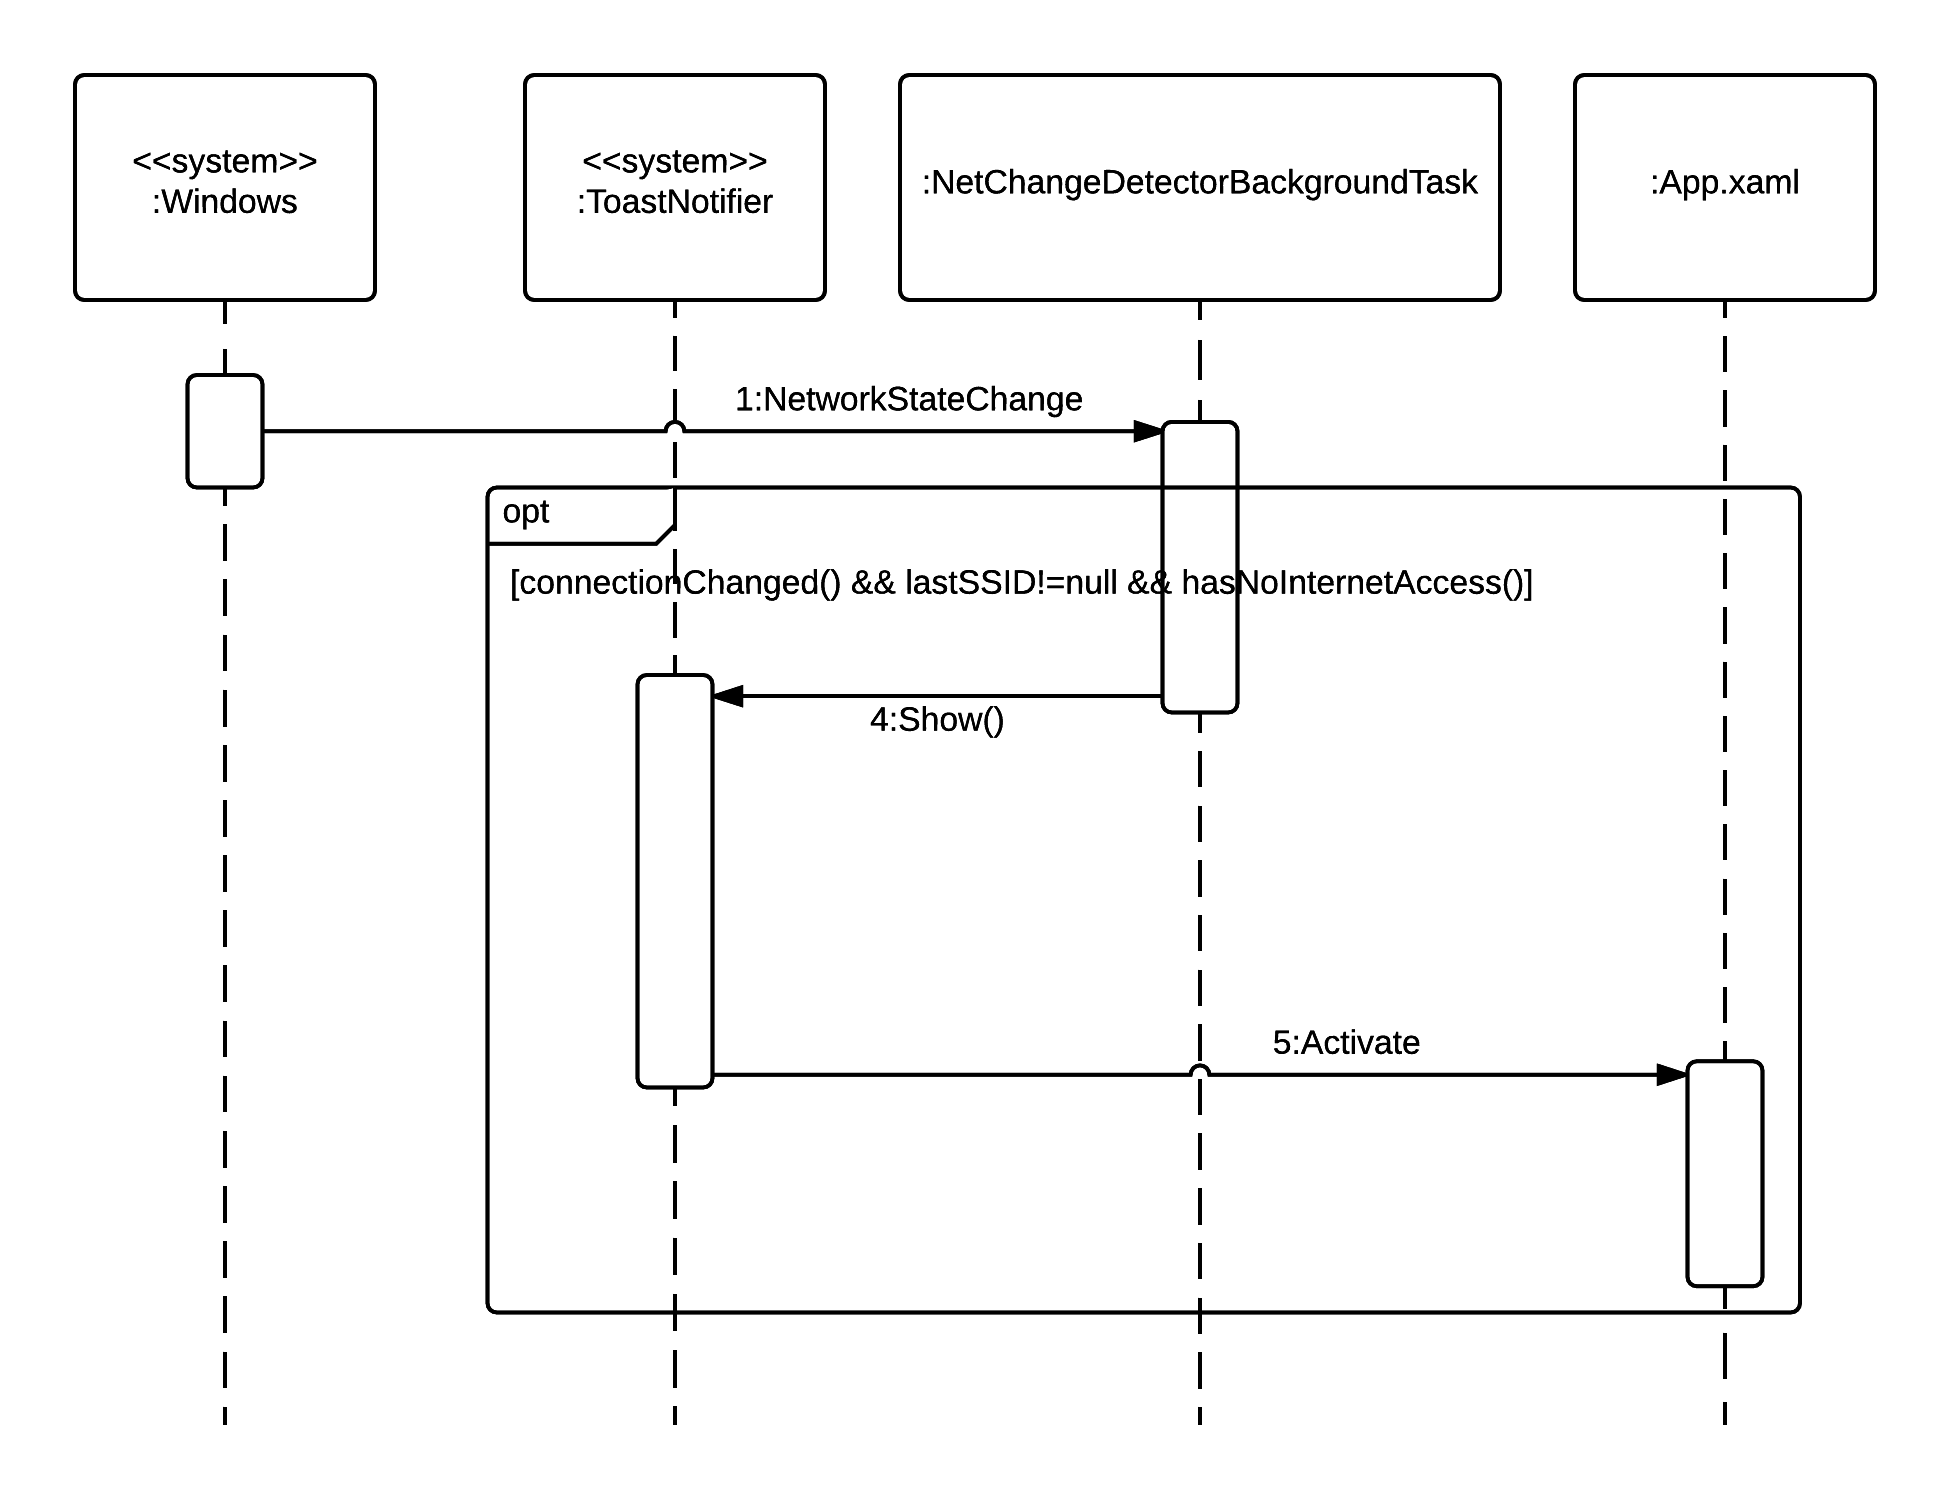
\includegraphics[scale=0.9]{Gambar/SequenceDiagramNetworkDetection.png}
    \caption[Diagram Interaksi Deteksi Jaringan.]{Diagram Interaksi Deteksi Jaringan.} 
    \label{fig:NetworkDetectionSequenceDiagram}
\end{figure}

Gambar \ref{fig:NetworkDetectionSequenceDiagram} menjelaskan mengenai interaksi antar objek dalam perangkat lunak untuk melakukan deteksi perubahan jaringan. Interaksi yang terjadi adalah sebagai berikut:

\begin{enumerate}
    \item{Saat komputer mengalami perubahan jaringan (tidak terhubung menjadi terhubung dan sebaliknya, atau terjadi perubahan \textit{cost} jaringan), \textit{trigger} NetworkStateChange akan diaktifkan oleh Windows, dan objek NetChangeDetectorBackgroundTask yang sudah didaftarkan akan menerima \textit{trigger} tersebut.}
    \item{Jika kondisi \texttt{connectionChanged() \&\& lastSSID!=null \&\& hasNoInternetAccess()} terpenuhi, maka:}
    \begin{enumerate}
        \item{NetChangeDetectorBackgroundTask memerintahkan ToastNotifier untuk memunculkan notifikasi menggunakan method Show().}
        \item{Saat user menekan tombol "Yes" pada notifikasi, App.xaml diaktivasi.}
    \end{enumerate}
\end{enumerate}

\subsection{Perancangan Interaksi Penciptaan Password}
\label{subsec:perancangan_interaksi_penciptaan_password}

\begin{figure}[!htb]
    \centering
    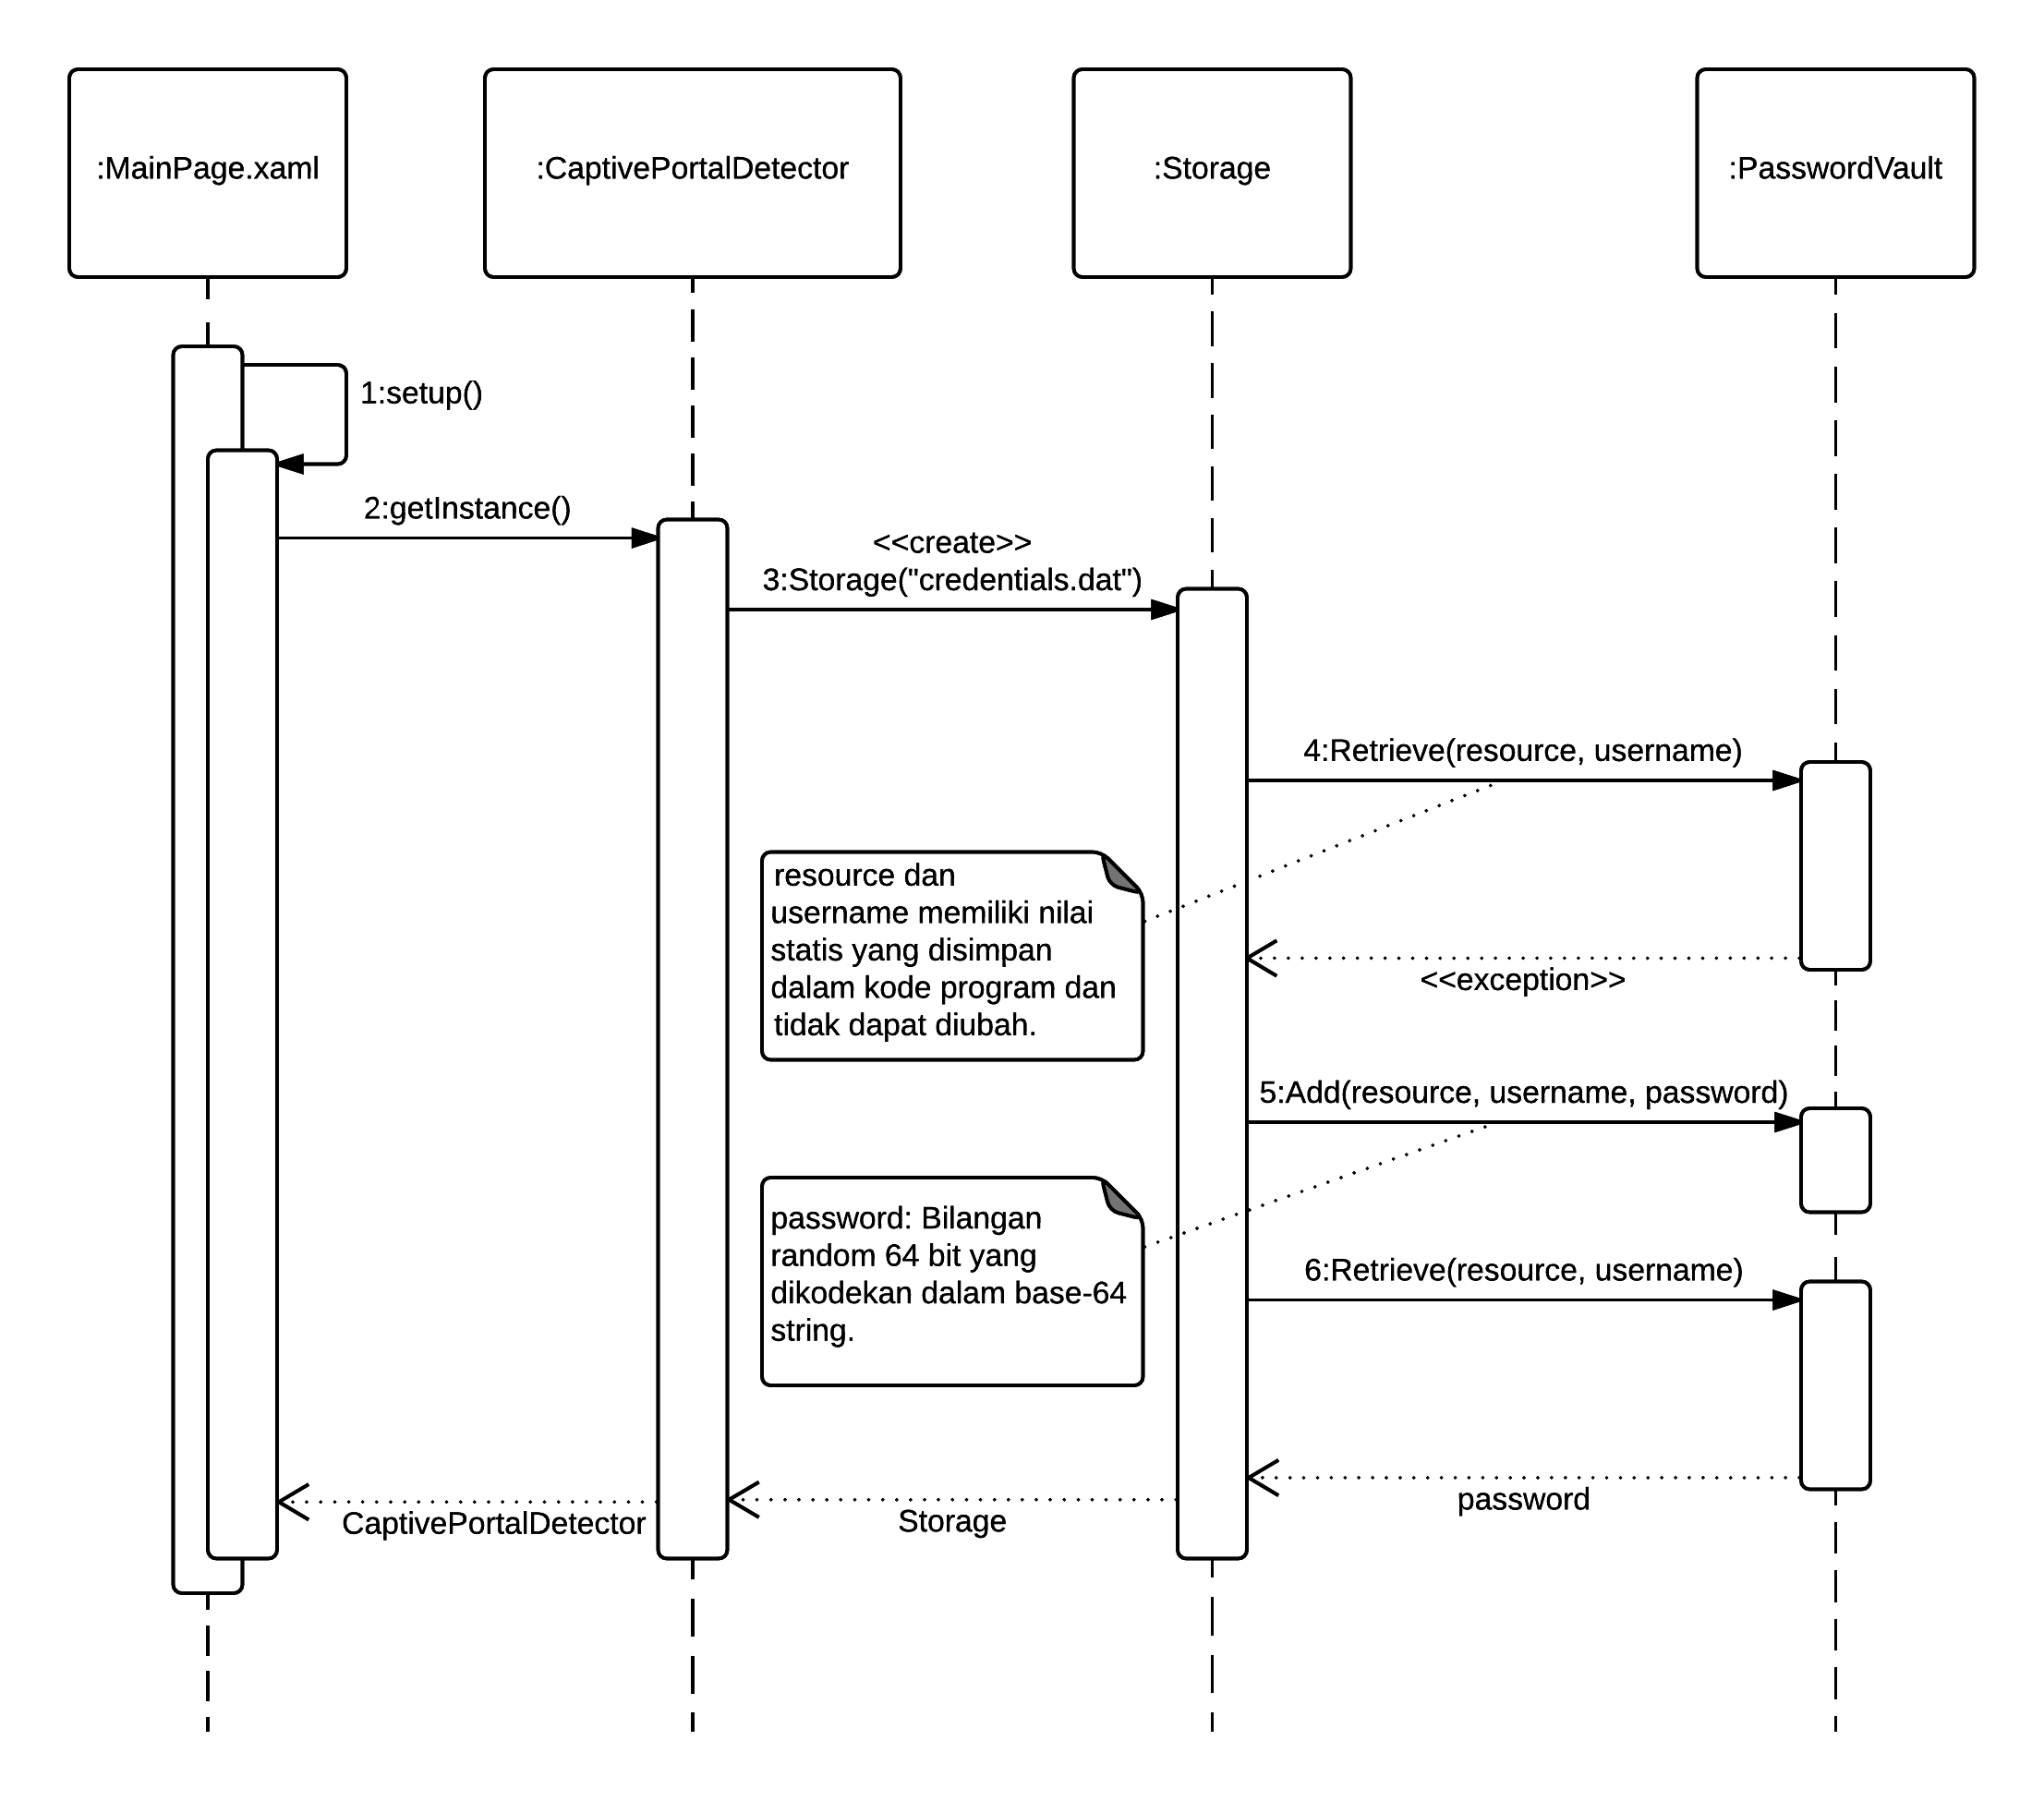
\includegraphics[scale=0.9]{Gambar/SequenceDiagramPasswordGeneration.png}
    \caption[Diagram Interaksi Penciptaan Password.]{Diagram Interaksi Penciptaan Password.} 
    \label{fig:PasswordGenerationSequenceDiagram}
\end{figure}

Gambar \ref{fig:PasswordGenerationSequenceDiagram} menjelaskan mengenai interaksi antar objek dalam perangkat lunak untuk menciptakan password random saat perangkat lunak pertama kali dijalankan. Interaksi yang terjadi adalah sebagai berikut:

\begin{enumerate}
    \item{MainPage.xaml melakukan setup().}
    \item{MainPage.xaml memanggil metode getInstance() pada CaptivePortalDetector untuk mendapatkan \textit{instance} CaptivePortalDetector.}
    \item{CaptivePortalDetector menciptakan objek Storage baru pada \textit{constructor}-nya.}
    \item{Objek Storage berusaha untuk mendapatkan password dengan memangil metode Retrieve() pada objek PasswordVault, namun mendapatkan exception karena belum ada password yang disimpan.}
    \item{Objek Storage memasukkan password baru yang diciptakan secara random menggunakan metode Add() pada PasswordVault.}
    \item{Objek Storage memanggil metode Retrieve() kembali pada objek PasswordVault, dan mendapatkan password yang baru saja diciptakan. Setelah itu, CaptivePortalDetector mendapatkan objek Storage, dan MainPage.xaml mendapatkan \textit{instance} CaptivePortalDetector.}
\end{enumerate}

\subsection{Perancangan Interaksi Penyimpanan Informasi Login}
\label{subsec:perancangan_interaksi_penciptaan_password}

\begin{figure}[!htb]
    \centering
    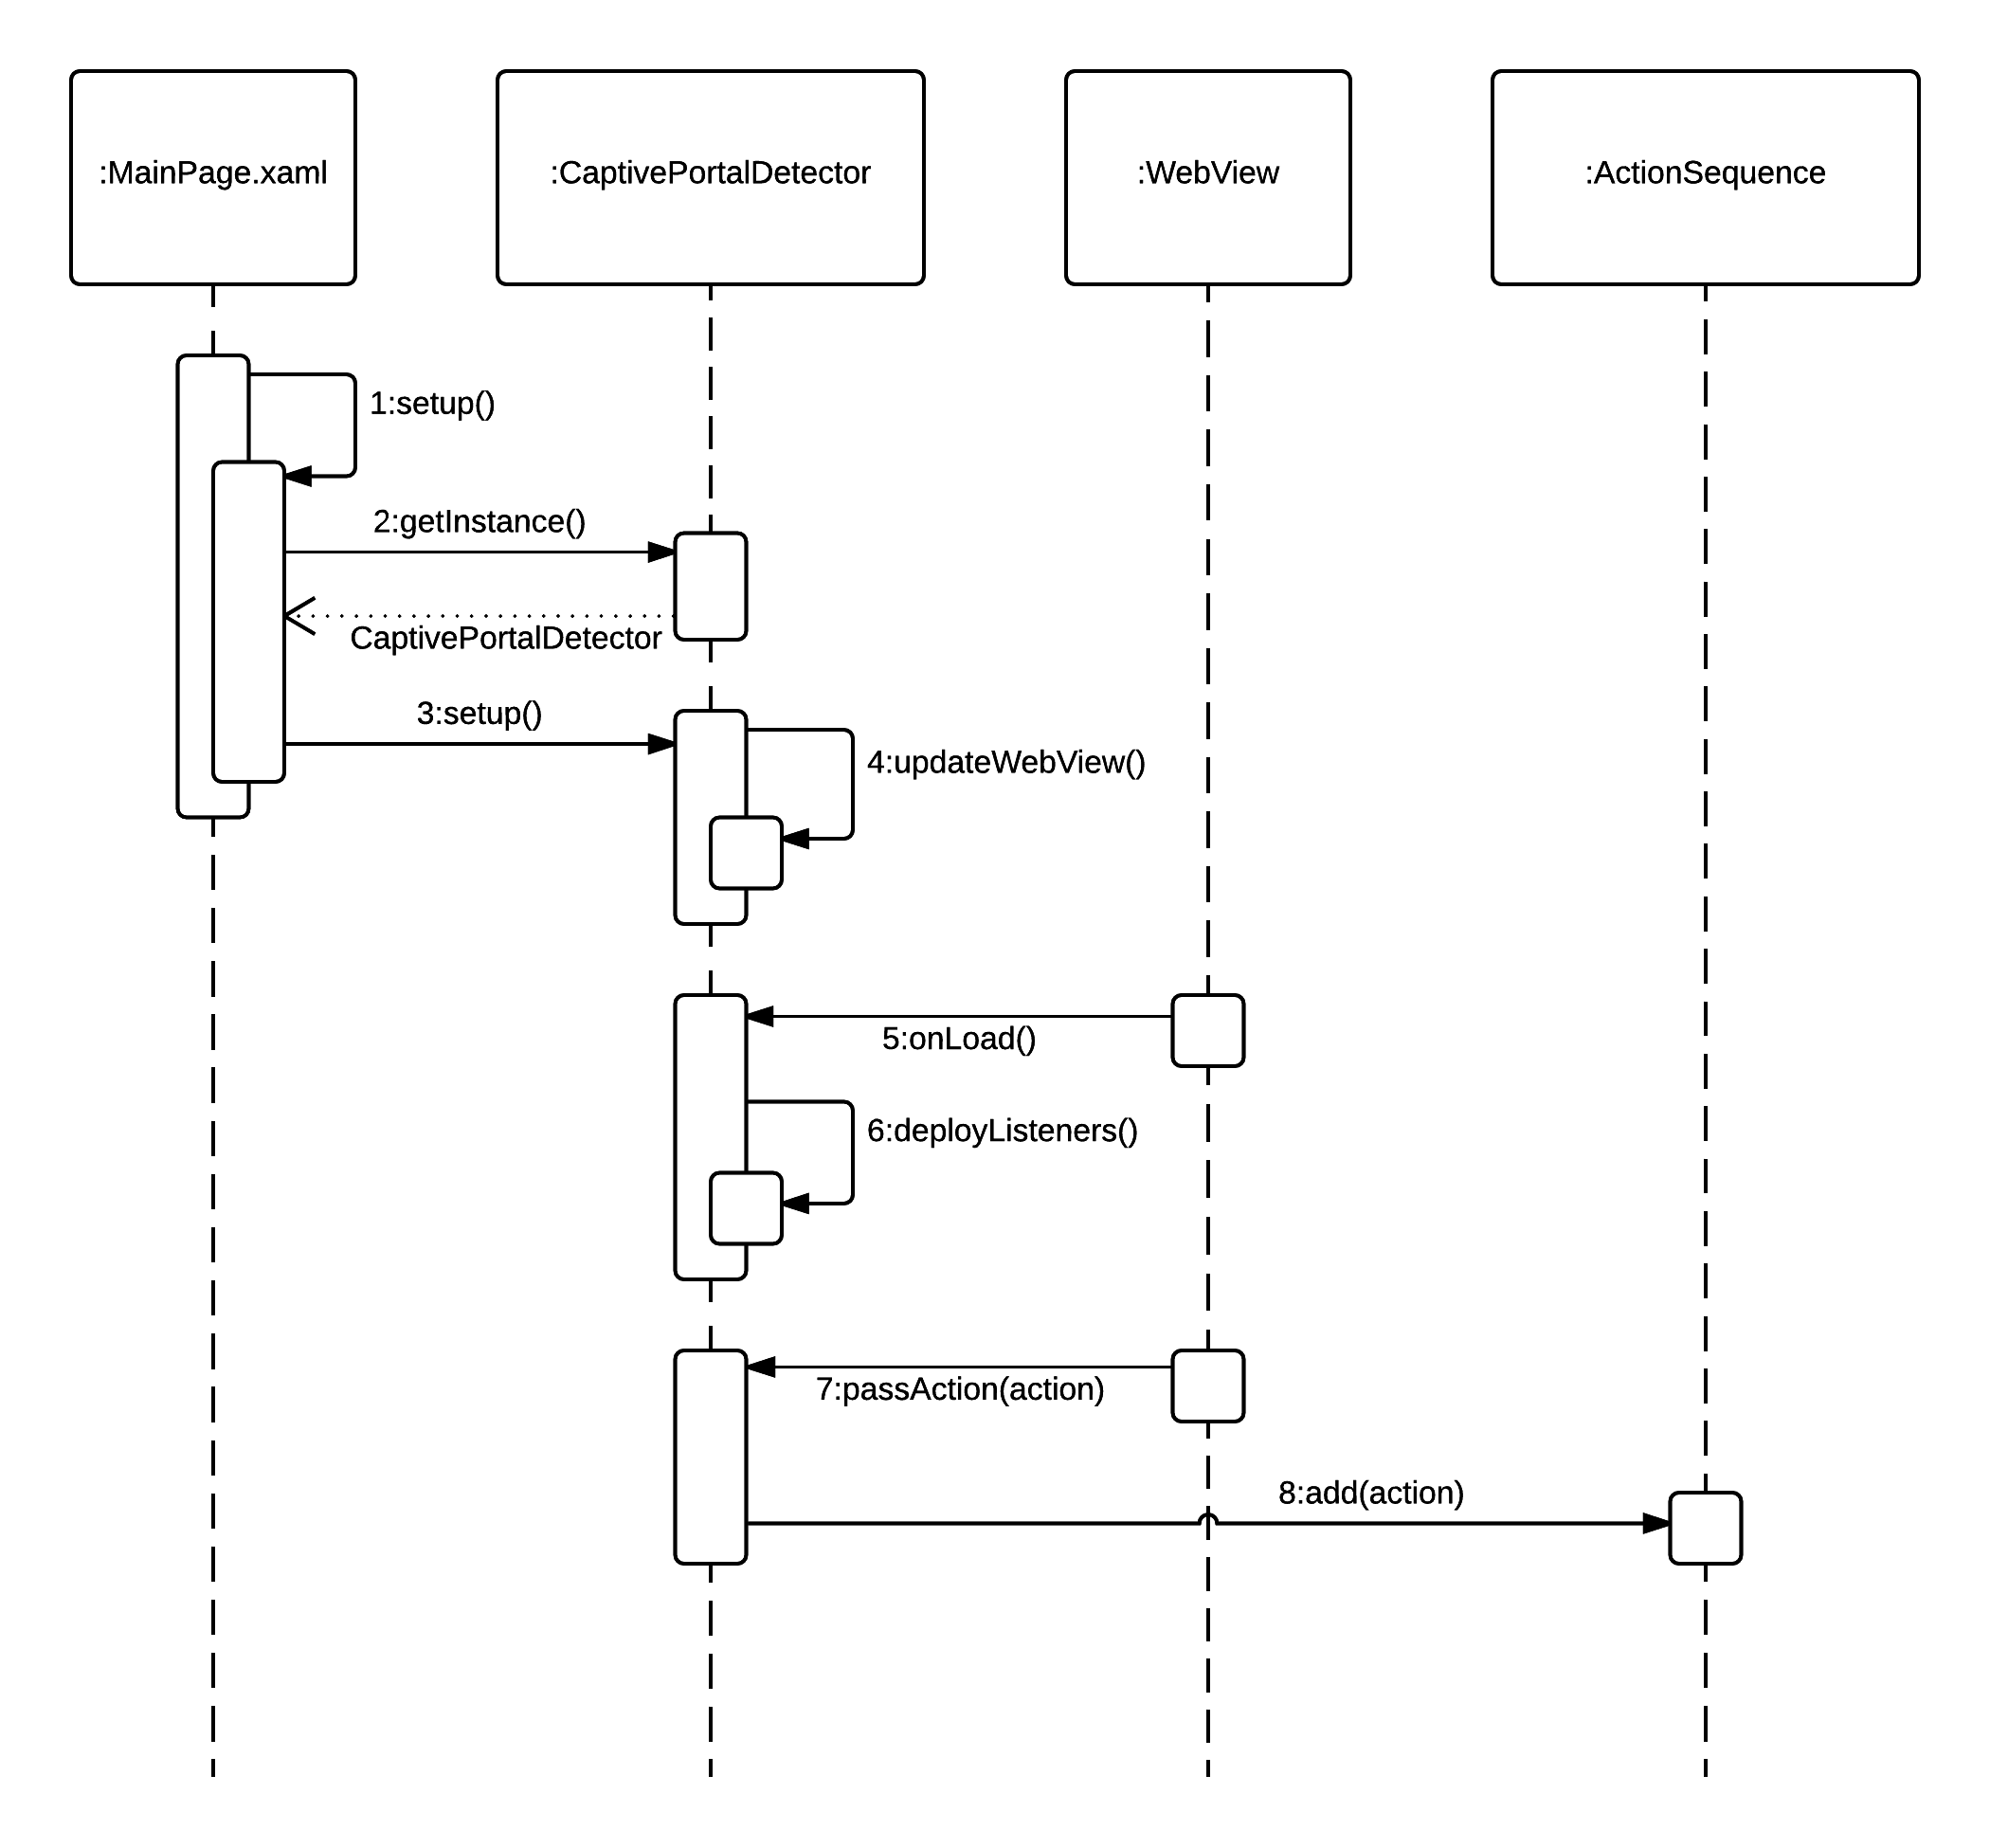
\includegraphics[scale=0.9]{Gambar/SequenceDiagramLoginInformationSaving.png}
    \caption[Diagram Interaksi Penyimpanan Informasi Login.]{Diagram Interaksi Penyimpanan Informasi Login.} 
    \label{fig:LoginInformationSavingSequenceDiagram}
\end{figure}

Gambar \ref{fig:LoginInformationSavingSequenceDiagram} menjelaskan mengenai interaksi antar objek dalam perangkat lunak untuk menyimpan informasi login. Interaksi yang terjadi adalah sebagai berikut:

\begin{enumerate}
    \item{MainPage.xaml melakukan setup().}
    \item{MainPage.xaml memanggil metode getInstance() pada kelas CaptivePortalDetector untuk mendapatkan \textit{instance} CaptivePortalDetector. MainPage.xaml mendapatkan \textit{instance} CaptivePortalDetector.}
    \item{MainPage.xaml memanggil metode setup() pada objek CaptivePortalDetector.}
    \item{CaptivePortalDetector melakukan updateWebView() untuk mengarahkan WebView ke URI yang digunakan untuk melakukan deteksi koneksi internet.}
    \item{WebView memanggil metode onLoad() pada objek CaptivePortalDetector saat halaman selesai dimuat.}
    \item{Jika halaman tidak berisi teks "connected" (tanpa tanda petik), CaptivePortalDetector melakukan deployListeners() untuk menangkap semua \textit{event} yang mungkin dilakukan oleh pengguna pada halaman tersebut.}
    \item{Metode passAction() dipanggil pada objek CaptivePortalDetector saat pengguna melakukan klik atau input teks untuk mengirimkan aksi yang baru saja dilakukan oleh pengguna.}
    \item{CaptivePortalDetector memanggil metode add() pada objek ActionSequence untuk menyimpan aksi tersebut.}
\end{enumerate}



\section{Perancangan Antarmuka}
\label{sec:perancangan_antarmuka}

Pengguna memerlukan antarmuka untuk berinteraksi dengan perangkat lunak. Antarmuka yang diperlukan adalah:

\begin{itemize}
    \item{Antarmuka notifikasi yang muncul setiap kali terhubung dengan WiFi yang menggunakan \textit{captive portal}.}
    \item{Antarmuka untuk menampilkan halaman web.}
    \item{Antarmuka untuk menampilkan pesan-pesan seperti pesan "Connected." atau "Check your network connection.".}
\end{itemize}

\subsection{Antarmuka Notifikasi}
\label{subsec:antarmuka_notifikasi}

\begin{figure}[!htb]
    \centering
    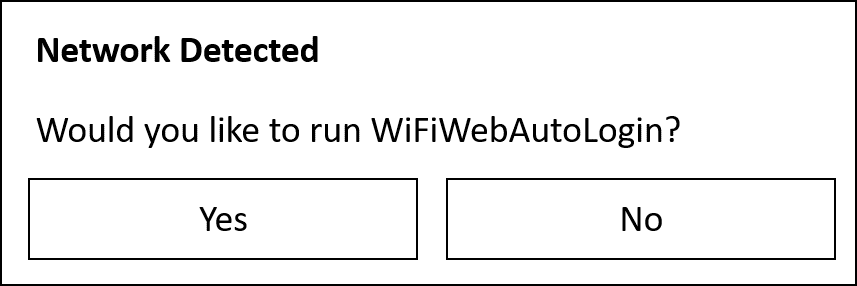
\includegraphics[scale=0.5]{Gambar/UI_Notification.png}
    \caption[Rancangan Antarmuka Notifikasi.]{Rancangan Antarmuka Notifikasi.}
    \label{fig:RancanganAntarmukaNotifikasi}
\end{figure}

Gambar \ref{fig:RancanganAntarmukaNotifikasi} menampilkan desain antarmuka notifikasi. Desain antarmuka notifikasi menggunakan desain notifikasi standar windows dengan dua tombol, "Yes" dan "No". Jika tombol "Yes" ditekan, maka notifikasi akan hilang dan aplikasi akan dijalankan. Jika tombol "No" ditekan, maka notifikasi akan hilang. Antarmuka notifikasi adalah antarmuka yang pertama kali akan muncul dalam siklus aplikasi karena kelas NetChangeDetectorBackgroundTask didaftarkan pada sistem untuk mendeteksi perubahan jaringan.

\subsection{Antarmuka Aplikasi}
\label{subsec:antarmuka_aplikasi}

Antarmuka untuk menampilkan halaman web dan menampilkan pesan dapat disatukan menjadi antarmuka aplikasi yang halaman kontennya dapat diubah menjadi WebView saat berada dalam mode web browser, dan menjadi Label saat berada dalam mode message box.

\subsubsection{Antarmuka Message Box}
\label{subsec:antarmuka_message_box}

\begin{figure}[!htb]
    \centering
    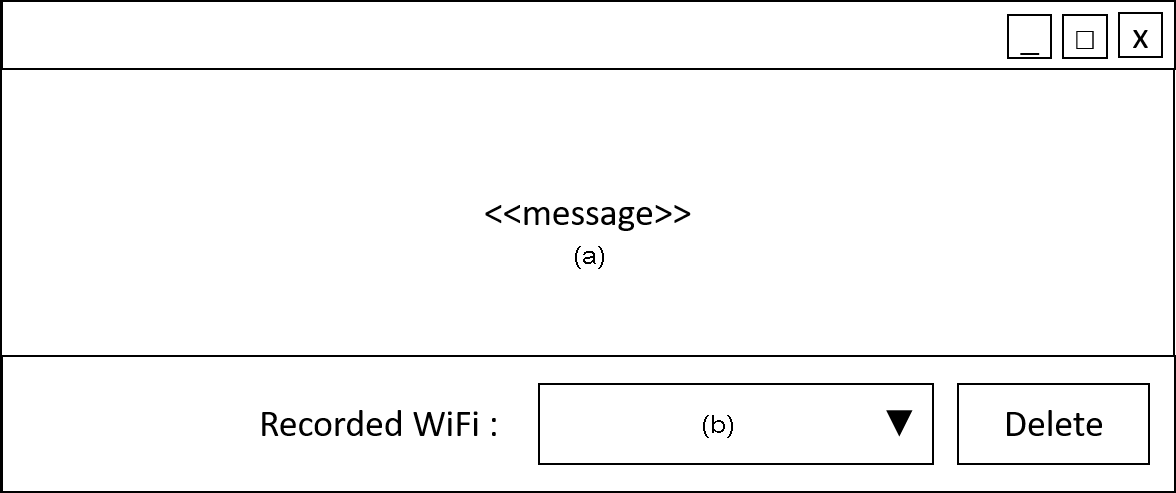
\includegraphics[scale=0.5]{Gambar/UI_MessageBox.png}
    \caption[Rancangan Antarmuka Message Box.]{Rancangan Antarmuka Message Box.}
    \label{fig:RancanganAntarmukaMessageBox}
\end{figure}

Gambar \ref{fig:RancanganAntarmukaMessageBox} menampilkan desain antarmuka message box. Selain label untuk menaruh pesan, antarmuka ini juga memiliki \textit{selector} untuk dapat menghapus WiFi yang sudah terekam. Dengan menghapus WiFi yang terdapat pada \textit{selector} ini, pengguna dapat merekam ulang informasi login pada WiFi tersebut.

\subsubsection{Antarmuka Web Browser}
\label{subsec:antarmuka_web_browser}

\begin{figure}[!htb]
    \centering
    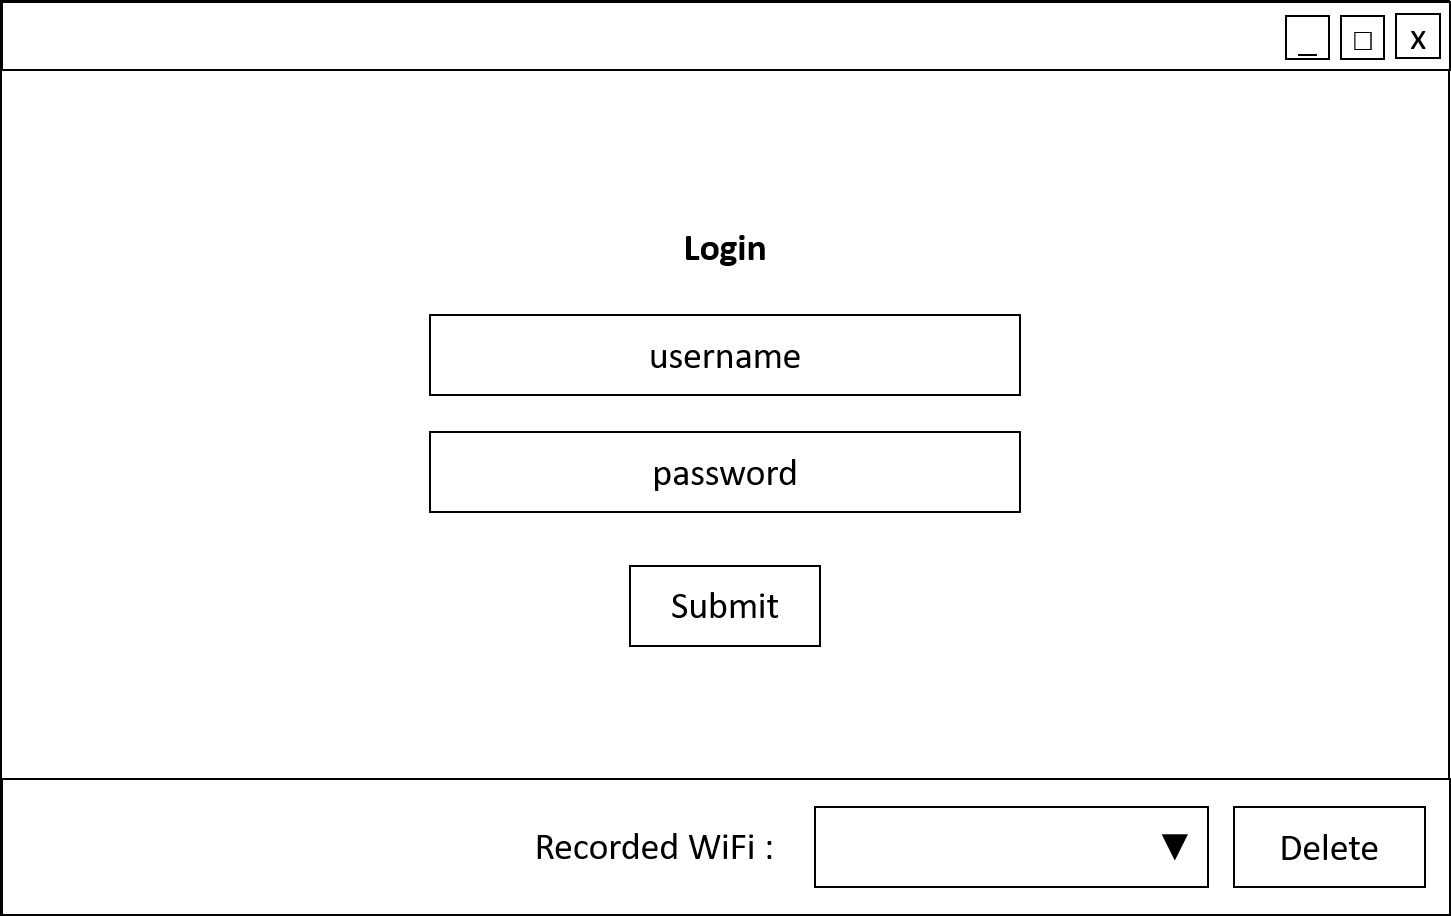
\includegraphics[scale=0.5]{Gambar/UI_WebBrowser.png}
    \caption[Rancangan Antarmuka Web Browser.]{Rancangan Antarmuka Web Browser.}
    \label{fig:RancanganAntarmukaWebBrowser}
\end{figure}

Gambar \ref{fig:RancanganAntarmukaWebBrowser} menampilkan desain antarmuka web browser. Antarmuka ini digunakan untuk menampilkan halaman web yang berkaitan dengan login \textit{captive portal}. Pada antarmuka inilah aksi pengguna akan direkam secara otomatis. Selain itu, pada antarmuka ini terdapat komponen yang sama dengan antarmuka message box, yaitu komponen \textit{selector} untuk menghapus SSID WiFi yang sudah terekam.